% !TEX root =  paper.tex
\section{Introduction}

% \begin{figure}[t!]
% 	\centering
% 	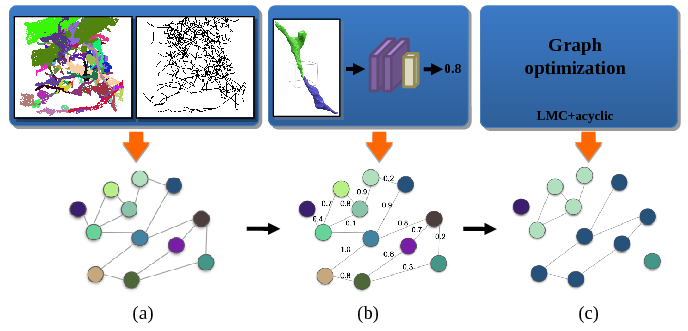
\includegraphics[width=\linewidth]{./figures/teaser_v2.png}
% 	\caption{Our proposed framework uses both local and global biological constraints to improve an input segmentation.}
% 	\label{fig:teaser}
% \end{figure}
\begin{figure}[t]
	\centering
	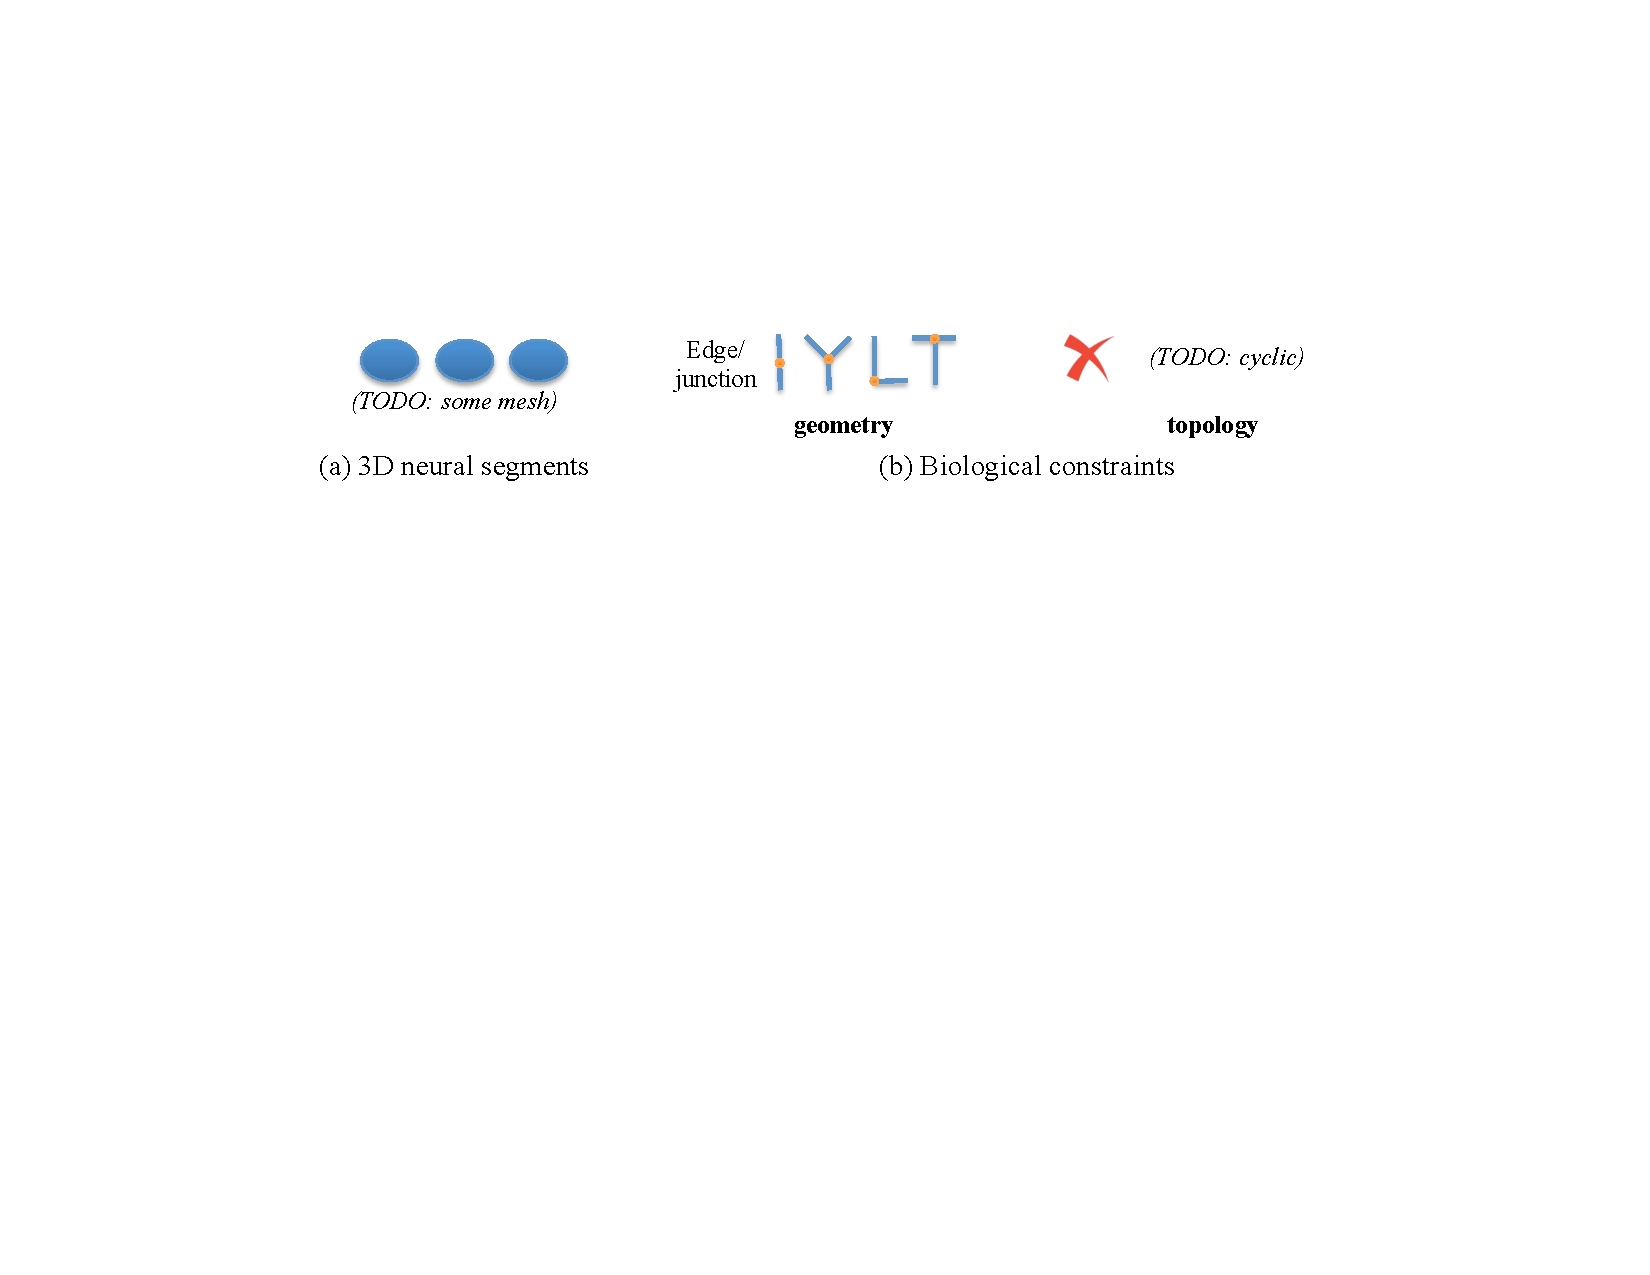
\includegraphics[width=\linewidth]{./figures/bc/teaser_bc_v2.pdf}
	\caption{Biological constraints for 3D segments in Connectomics.}
	\label{fig:bc}
\end{figure}


The field of connectomics is concerned about reconstructing the wiring diagram of the brain at nanometer resolutions to enable new insights into the workings of the brain~\cite{haehn2017scalable,kasthuri2015saturated}. 
%Recent advancements in image acquisition using multi-beam serial-section electron microscopy (sSEM) allow researchers to produce terabytes of image data per hour~\cite{hildebrand2017whole}. 
%It is infeasible for domain experts to manually reconstruct this vast amount of image data~\cite{haehn2014design}. 
State-of-the-art automatic 3D reconstruction approaches use pixel-based convolutional neural networks (CNNs) and watershed transform to generate initial segmentation, followed by agglomeration steps~\cite{seymour2016rhoananet,lee2015recursive,nunez2014graph,parag2017anisotropic,ronneberger2015u,zlateski2015image}.
%These \textit{bottom-up pixel-based} methods produce excellent results but still fall short of acceptable error rates for large volumes.
For the agglomeration, most methods do not make use of the biological knowledge of the 3D shape of neural structures.
Reported on small-sized volumes, a simple threshold-based mean agglomeration method can achieve superhuman result~\cite{lee2017superhuman}.
However, it is unclear if it is the case for larger volumes.


%\TODO{the selling point is to add biological constraint}
%We present a \textit{top-down graph-based} method that builds on the outputs of bottom-up pixel-based segmentation approaches. 
We here present a new agglomeration method that imposes both local and global biological constraints onto the output segmentation to match the underlying structure of neuronal processes.
We first extract skeletons from labels in the input segmentation and generate a simplified graph (Fig.~\ref{fig:teaser}a). 
Next, we train a CNN classifier to learn biological constraints on the local structural shape of a neuron (Fig.~\ref{fig:teaser}b). 
This classifier produces probabilities that two segments belong to the same neuron based on the input shapes of the segments.
These probabilities correspond to edge weights in our graph extracted from the input segmentation.
We then use a graph optimization algorithm to partition the graph into a final improved reconstruction by enforcing domain-specific topological constraints from biology (Fig.~\ref{fig:teaser}c).

%Our approach operates at a level of abstraction above existing pixel-based methods. 
%This allows us to leverage both local and global information to produce more accurate reconstructions. 
With the biological constraints, we can make use of both geometric and topological prior information to produce more accurate reconstructions.
\TODO{refer to figure 1}
Our method is independent of image resolution and acquisition parameters, enabling its application to isotropic and anisotropic image data without retraining.
Images generated by electron microscopes often differ in appearance because of variations in staining techniques \cite{briggman2012volume}.
By removing the dependence of our algorithm on the input images, we greatly reduce the need for additional costly ground truth data for each new stack of images.
Using the graph induced by the segmentation allows us to enforce global biological constraints on the reconstruction. 
Our dual approach of assessing local decisions in a global context yields accuracy improvements over existing reconstruction methods.


This work makes three contributions.
First, a novel top-down framework that extracts graphs from skeletonized 3D segmentations for improved neural reconstruction of connectomics data; 
Then, a region-based CNN classifier to detect errors; 
%(3) an empirical evaluation of our method on several connectomics datasets;  % this is not contribution
Last, improved performance over a state-of-the-art pixel-based reconstruction approach on average by \TODO{XX}\% with suitable running times.
